\section{Results}
\label{sec:results}

% ==========================================================================
% Table 1 (AIAS 2026 workshop copy; caption shortened by
% analysis/scripts/mk_table_collapse_ws.py) -- functional collapse per actor, compact form
%
% GENERATED FILE -- do not edit by hand. Any edit is overwritten.
% generating script : analysis/scripts/mk_tables.py
% canonical input   : analysis/out/FINAL_TABLES_OUTPUT.txt  sections T1, T23
%                    analysis/out/FIGDATA_BF.json  (role-free with feedback: collapse only)
% frozen data       : experiments/results/FROZEN/, frozen_at 2026-09-30T10:09:30.201557
%                     11600 trajectories
%                     sha256 fa22a446d5314bb67b1c6a6444b511eeeae3eb8770419a36f182617eeccbf3b5  actor3.jsonl
%                     sha256 038e08aec4d4aee166106a6325309dfe2301faf339c7d0bf82338a74576424d4  armCp.jsonl
%                     sha256 e4e53cb117d91129991ce2fe87e336e152fc9ee6ca826d363f2bd5dd240d7130  campaign_v2.jsonl
% canonical-output sha256 : b26ccb5451a5eaed14046a27a980ba8797e5669912df907bc25f69bf60ad5b76
% generation date   : 2026-10-04  (derived from the canonical
%                     input's mtime, not wall-clock: regeneration must
%                     be byte-identical)
%
% Compact form of the supplement's full collapse table
% (supp_role_collapse.tex): byte duplication, the enforced row and the
% marker sensitivity live there, built from the same parsed inputs.
% The adjudication is outcome-blind but NOT condition-blind: do not
% describe it as blinded (APPROVED_CLAIMS A1 / DEAD list).
%
% Reader-facing condition names per paper/TERMINOLOGY.md; internal arm
% codes are deliberately absent and their absence is asserted at
% generation time.
% ==========================================================================
\begin{table}[t]
\centering
\caption{\textbf{Functional collapse on the Omni-MATH benchmark.} Share of
first cycles (the first pass of the three agents) in which all three assert
their own final answer, per actor; bold: without roles. RS: role-structured; RF$^{-}$ and RF: role-free with the evaluator's
feedback withheld or shown. \emph{Adjudicated no division}: share of a
judged sample of first cycles in which a model judge with a fixed rubric
(outcome-blind, not condition-blind) finds no division of labor.}
\label{tab:collapse}
\small
\begin{tabular}{@{}l ccc cc@{}}
\toprule
 & \multicolumn{3}{c}{functional collapse} & \multicolumn{2}{c}{adjudicated no division} \\
\cmidrule(lr){2-4}\cmidrule(lr){5-6}
actor & RS & RF$^{-}$ & RF & RS & RF$^{-}$ \\
\midrule
gemma-4-31B & $0.000$ & $\mathbf{0.976}$ & $\mathbf{0.974}$ & $0.000$ & $\mathbf{0.857}$ \\
gpt-oss-120b & $0.120$ & $\mathbf{0.846}$ & $\mathbf{0.883}$ & $0.000$ & $\mathbf{1.000}$ \\
Llama-3.3-70B & $0.000$ & $\mathbf{0.872}$ & $\mathbf{0.900}$ & $0.000$ & $\mathbf{1.000}$ \\
\bottomrule
\end{tabular}
\end{table}


\begin{figure}[t]
\centering
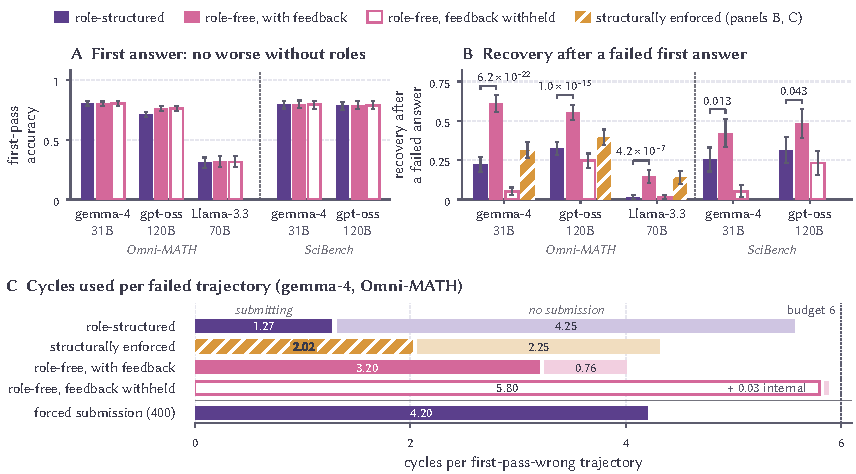
\includegraphics[width=\textwidth]{figures/fig1_v3_story_ws.pdf}
\caption{\textbf{Roles organize the team; the Reviewer's gate limits feedback and recovery.}
\textbf{(A)} First-pass accuracy, over trajectories with a first verdict.
\textbf{(B)} Recovery: the share of first-pass-wrong trajectories (first
graded answer wrong) that finish correct, each condition over its own set; brackets give the exact
McNemar $p$ for role-structured against role-free with feedback, paired on
problems both first answer wrongly. \textbf{(C)} Cycles of gemma-4's first-pass-wrong Omni-MATH
trajectories that end in a submission (the third agent approved) or
internally (it declined); a PASS ends a
trajectory early. Hollow bars: role-free with feedback withheld, a diagnostic. In (B),
enforced trajectories that never finish count as unrecovered.
Bottom row: the
exploratory forced-submission run ($400$ problems). Error bars: bootstrap
$95\%$ intervals.}
\label{fig:dissociation}
\end{figure}

\subsection{R1. Roles create specialization, but not a better first
answer}
\label{subsec:collapse}

Removing role instructions largely eliminates the intended division of
labor for all three actors (gemma-4, gpt-oss and Llama-3.3) on the
Omni-MATH benchmark: functional collapse, the share of first cycles in
which every agent asserts its own final answer, is rare with roles and the
norm without them (Table~\ref{tab:collapse}). The change comes mostly from the Planner; the Executor answers either way. A role-structured
Planner seldom states an answer and a role-free one nearly always does, so the division of labor rests on a single \textsc{must not} clause. Because the role-free footer asks for an answer, the absolute level
partly reflects that request, but the ordering holds under all three
answer-marker definitions, the cues that count as an answer
(Appendix~\ref{sec:collapse_full}). A model judge, outcome-blind but not condition-blind, agrees in direction (Table~\ref{tab:collapse}).

Despite this loss of specialization, first-pass accuracy is largely
unaffected. On problems graded under both conditions, using the frozen feedback-withheld cells, whose inputs equal the role-free team's with feedback
until the first verdict, it is unchanged for gemma-4 and Llama-3.3 and
higher without roles for gpt-oss (Figure~\ref{fig:dissociation}A;
Table~\ref{tab:recovery}). Because one model plays every agent, a Planner
that solves the whole problem brings no competence the Executor lacks;
gpt-oss may gain from extra independent solutions
(Appendix~\ref{app:results}).

\subsection{R2. With equal feedback access, the role-free team recovers more}
\label{subsec:recovery}

%% GENERATED by analysis/scripts/mk_table_main.py --workshop from
%% FIGDATA_BF.json and FIGDATA_GATE.json -- do not edit by hand.
\begin{table}[t]
\centering
\caption{\textbf{Role-structured against role-free with feedback, in every cell} (one actor
on one benchmark; $n$ problems). RS: role-structured; RF: role-free with
the evaluator's feedback shown; RF$^{-}$: role-free with it withheld, a
diagnostic. A trajectory is first-pass wrong when its first graded answer is wrong: its
first submission, or the single end-of-budget grading if it never submits.
\emph{Recovery}: share of first-pass-wrong trajectories that finish
correct, each over its own set. \emph{Recovered only by}: on the $n$
problems both first answer wrongly, those recovered by one condition only,
with the exact McNemar $p$. \emph{Verdict-matched} (post hoc): the same,
with each RF trajectory cut off after as many verdicts as RS received.
\emph{Final accuracy}: over all problems, paired. \emph{Submissions}:
third-agent approvals per first-pass-wrong trajectory. \emph{RS never
submits}: RS first-pass-wrong trajectories with no submission in six
cycles.}
\label{tab:main}
\footnotesize
\setlength{\tabcolsep}{5pt}
\begin{tabular}{@{}l ccc cccc@{}}
\toprule
 & \multicolumn{3}{c}{recovery} & \multicolumn{4}{c}{recovered only by (paired)} \\
\cmidrule(lr){2-4}\cmidrule(lr){5-8}
actor, domain ($n$) & RS & RF & RF$^{-}$ & $n$ & RS & RF & $p$ \\
\midrule
gemma-4, Omni-MATH ($1{,}600$) & $0.222$ & $0.609$ & $0.051$ & $236$ & $4$ & $89$ & $6.2{\times}10^{-22}$ \\
gpt-oss, Omni-MATH ($1{,}600$) & $0.324$ & $0.552$ & $0.247$ & $319$ & $17$ & $101$ & $1.0{\times}10^{-15}$ \\
Llama-3.3, Omni-MATH ($400$) & $0.014$ & $0.147$ & $0.015$ & $250$ & $1$ & $26$ & $4.2{\times}10^{-7}$ \\
\addlinespace
gemma-4, SciBench ($574$) & $0.254$ & $0.419$ & $0.051$ & $100$ & $7$ & $21$ & $0.013$ \\
gpt-oss, SciBench ($574$) & $0.315$ & $0.483$ & $0.231$ & $93$ & $7$ & $18$ & $0.043$ \\
\bottomrule
\end{tabular}

\medskip
\begin{tabular}{@{}l ccc ccc cc c@{}}
\toprule
 & \multicolumn{3}{c}{verdict-matched} & \multicolumn{3}{c}{final accuracy}
 & \multicolumn{2}{c}{submissions} & RS never \\
\cmidrule(lr){2-4}\cmidrule(lr){5-7}\cmidrule(lr){8-9}
actor, domain ($n$) & RS & RF & $p$ & RS & RF & $p$ & RS & RF & submits \\
\midrule
gemma-4, Omni-MATH ($1{,}600$) & $0.165$ & $0.153$ & $0.69$ & $0.846$ & $0.921$ & $1.7{\times}10^{-24}$ & $1.27$ & $3.20$ & $84/316$ \\
gpt-oss, Omni-MATH ($1{,}600$) & $0.229$ & $0.216$ & $0.72$ & $0.803$ & $0.894$ & $2.7{\times}10^{-28}$ & $2.10$ & $3.53$ & $51/463$ \\
Llama-3.3, Omni-MATH ($400$) & $0.012$ & $0.008$ & $1.0$ & $0.315$ & $0.415$ & $1.6{\times}10^{-7}$ & $0.32$ & $2.71$ & $205/276$ \\
\addlinespace
gemma-4, SciBench ($574$) & $0.230$ & $0.190$ & $0.48$ & $0.847$ & $0.880$ & $0.0054$ & $1.95$ & $3.62$ & $3/118$ \\
gpt-oss, SciBench ($574$) & $0.215$ & $0.247$ & $0.68$ & $0.852$ & $0.892$ & $1.9{\times}10^{-4}$ & $2.68$ & $3.95$ & $1/124$ \\
\bottomrule
\end{tabular}
\end{table}


The two teams diverge after a rejected first answer. In this main
comparison, exploratory because it was added after the freeze
(\S\ref{subsec:prereg}), the role-free team recovers more in all five cells (Table~\ref{tab:main}), both over its own failed
trajectories and, paired, on the problems both teams first answer wrongly.
For the gemma-4 model on Omni-MATH, it recovers $0.609$ of its failed
trajectories against $0.222$ (Figure~\ref{fig:dissociation}B).

For gemma-4, both teams reach the same first-pass accuracy and, because a
PASS ends the trajectory, keep every correct first answer, so the extra recoveries carry straight into final accuracy.
In every cell, final accuracy is higher without roles. The recoveries are revisions: nearly every passing
answer differs from the one first rejected (Appendix~\ref{sec:recovery}).
Hints contain the gold answer verbatim in at most $2.3\%$ of failing
verdicts in any cell; we did not audit partial leakage. A second run of the
two gemma-4 cells with feedback is close to the first, though the SciBench
paired test weakens to $p=0.052$ (Appendix~\ref{app:results}). R3 asks
whether the gap reflects how well each team uses a verdict or how many
verdicts it draws.

\subsection{R3. The Reviewer's approval governs feedback opportunities}
\label{subsec:mechanism}

Every submission returns a verdict and, on a FAIL, a repair hint, so each
one is another chance to revise; the two teams differ in how often they
take it. For the gemma-4 model on the Omni-MATH benchmark, the
role-structured team submits $1.27$ times per failed trajectory against
$3.20$ for the role-free team (Figure~\ref{fig:dissociation}C), and it submits less often in every cell. Much of this
withholding happens before any feedback exists, and some failed trajectories never submit, so they never see external feedback
(Table~\ref{tab:main}). On
Omni-MATH, the prompt clause that forbids approval after a FAIL
covers only a minority of the declines for every actor, and in the cycles
it does not cover the Reviewer declines more often than the role-free
team's third agent, by far for gemma-4 and Llama-3.3 (Table~\ref{tab:gate}). The gate therefore
reflects the Reviewer's disposition rather than the letter of its prompt,
plausibly because an agent told to critique searches for flaws.

\paragraph{Removing the gate restores recovery.} To test whether the gate
causes the gap, we kept the role-structured prompts unchanged but submitted
the team's answer in every cycle, overriding the Reviewer. We ran this
exploratory test once, for gemma-4 on the $400$ Omni-MATH problems of a
post-freeze re-run of the role-structured condition
(Appendix~\ref{app:details}). Every cycle then becomes a submission
(Figure~\ref{fig:dissociation}C), and recovery rises from
$0.198$ in that re-run to $0.613$, matching the role-free team on the same
problems (Table~\ref{tab:forced}). First-pass accuracy does not move, so the Reviewer's early declines bought no better first answer but cost
chances to repair it.

\paragraph{At equal verdict counts, the gap disappears.} In a post hoc
comparison on the problems both teams first answer wrongly, we cut each
role-free trajectory after as many verdicts as the role-structured team
received. No cell then shows a significant difference
(Table~\ref{tab:main}), and the pooled difference is $+0.009$ $[-0.014,+0.033]$ in favor of roles. The matching is coarse: a
role-free trajectory cut after a single FAIL cannot recover, so wherever
the role-structured team received one verdict the pair ties at zero, as in
most of gemma-4's pairs. On problems with at least two verdicts the difference remains not significant.
Recoding the scoring defect of \S\ref{sec:limitations} gives roles a small
significant margin on all paired problems, and no variant puts the role-free team significantly ahead
(Table~\ref{tab:robust}). A truncation cannot show that the two teams use
each verdict equally well, but together with the forced-submission run it
indicates that the gap stems mainly from how often the team requests
feedback rather than from how well it uses that feedback.

\paragraph{Without feedback, submitting more does not help.} For gemma-4, with the feedback withheld, the role-free team still
submits in almost every cycle
(Figure~\ref{fig:dissociation}C) but repeats its answer, a single distinct answer in $84.5\%$ of its failed trajectories
($20.8\%$ for gpt-oss; Table~\ref{tab:enforcement}), and rarely recovers;
adding the verdict and hint to the otherwise identical prompts lifts its
recovery (Table~\ref{tab:main}). Against this diagnostic alone, roles would appear load-bearing for repair, clearly so only for gemma-4
(Table~\ref{tab:recovery}).

\subsection{R4. Generality and organizational constraints}
\label{subsec:xdomain}

\paragraph{The pattern recurs on a second domain.} On the text-only slice
of the SciBench benchmark (free-response college science problems), where only the domain wording of the prompts changes,
the gemma-4 and gpt-oss models show the same ordering in recovery and final
accuracy (Table~\ref{tab:main}). The recovery contrast is weaker,
consistent with a looser gate: the role-structured team almost always
submits at least once, and the contrast again vanishes at equal verdict
counts.

\paragraph{Enforcement loosens the gate but is brittle.}
\label{subsec:enforce} On Omni-MATH, with roles enforced through typed message formats, the
Planner never asserts a final answer in the first cycle, whereas it nearly
always does without roles. The enforced team also submits more often,
and where the gate was tightest, for the Llama-3.3 model, recovery rises
close to the role-free team's; for gemma-4 and gpt-oss the direction is the
same but not significant (Appendix~\ref{sec:enforcement}). The gain does not
reach end-to-end accuracy, because $8\%$ to $17\%$ of enforced trajectories
exhaust the allowed regenerations on malformed outputs and never finish.
Under the pre-registered rule, which counts them as incorrect, enforcement
lowers accuracy significantly for gemma-4 and leaves it unchanged for the other two; scoring only the trajectories that finish would suggest
gains for every actor, a survivorship bias (Appendix~\ref{app:results}). In
our implementation, enforcement thus trades one obstacle for another: it loosens the gate but adds a new way to fail.
